The current section focuses on how we can extend our reductions
to \textit{SourceOrExcess}. In the previous sections,
we gave an overview on how we can go from an \textit{EndOfLine} problem
to a topological problem. In the current section, we show how we can extend the idea
for the \textit{SourceOrExcess} problem. We hope by parsimoniously reducing the
\textit{SourceOrExcess} problem to a topological problem, it will lead
to future reductions to the \textit{PureCircuit}.

\subsubsection{Current Variants of the problem}
% TODO
\subsubsection{Going to 2-indegree}


% TODO: Fix references
In section {}, when talking about the \textit{StrongSperner} problem,
we observed how coloured subspaces may lead to many duplicated solutions.
Here, we are slightly modifying the definition of \textit{3D-StrongSperner}
in order to take advantage of that. We will then show how the above modification
can lead to parsimonious reductions.


\begin{definitionbox}{\textit{3D-CountingSS} problem definition}{3d-counting-ss}
    \textbf{Input}: A hazard-free colouring circuit $\lambda: (\{0,1\}^k)^3 \to \{-1,+1\}^3$ which
    follows the boundary conditions of the \textit{StrongSperner} problem as explained in \ref{def:strong-sperner}.

    \textbf{Output}: A coordinate $p= (i\bot, j\bot, k\bot) \in (\{0,1\}^k)^3$ such that
    $\lambda(p) = \bot^3$.
    If there exists $p = (ib_1, jb_2, kb_3)$ for some $b \in \{0,1, \bot\}^3 \smallsetminus \{\bot^3\}$,
    if $\lambda(p)= \bot^3$.
    Given $H =\{\textbf{Cube}(p) \mid p \in (\{0,1\}^k \smallsetminus \{1^k\})^3 \}$
    then all cubes in $\{A \in H \mid \textbf{Res}(A) \subset A \}$ count as $1$ solution.
\end{definitionbox}


% TODO: Add interpretation with directional values
The above idea is a natural extension of the \textit{StrongSperner} interpretation, where
its labelling represents the direction of a continuous function. If a face
of a cube is panchromatic, then that implies that there has to be a fixed point somewhere,
as seen in the figure \ref{fig:chap-3:panc-edge}. If an edge were to be panchromatic,
then that means that a fixed point could lie on the edge. If we were treating this as a
fixed point problem instead of a colouring one, it would make sense to argue that we have one solution.
We abuse this notion to argue that if a subspace of a cube is a solution, then we count all neighbouring
cubes as one individual solution.



\begin{figure}
    \centering
    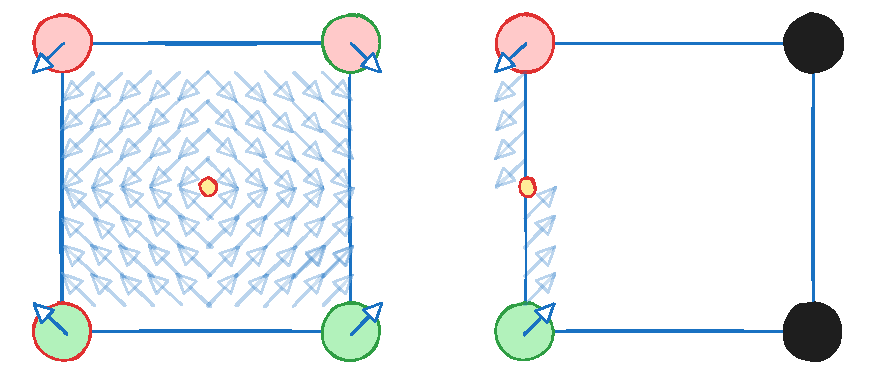
\includegraphics[width=0.7\textwidth]{Chapter3/edge-colouring.pdf}
    \caption{Panchromatic edge for 2 dimensions}
    \label{fig:chap-3:panc-edge}
\end{figure}

To prove \textbf{PPAD}-completeness, we know that the above problem can be reduced to \textit{3D-StrongSperner},
although the reduction will not be parsimonious. We now show the main result of our section:

\begin{theorembox}{Parsimonious reduction from $\textit{SourceOrExcess}(2,1)$}{}
    $$
        \textbf{\#PPAD}(\textit{SourceOrExcess}(2,1)) \subseteq
        \textbf{\#PPAD}(\textit{3D-CountingSS})
    $$
\end{theorembox}

\begin{proof}
    We will try and simplify a source or excess graph using the following table

    ![[1752512630-sourceorexcess-to-purecircuit 2025-07-15 11.38.39.excalidraw]]

    Where we essentially create transformation from $\{ 0,1 \}^n \to \{ 0,1 \}^{n+1}$. We create the following lemma

    > [!lemma] SourceOrExcess Transformation
    > Given $S, P_{1}, P_{2} \in \{ 0,1 \}^n \to \{ 0,1 \}^n$ , we can create $S', P'_{1}, P'_{2} \in \{ 0,1 \}^{n+1} \to \{ 0,1 \}^{n+1}$ that describe
    > the above transformations in poly-time

    `\begin{proof}`
        We argue that the following description of a circuit, recreates our transformations:
        * We default all $1b$ where $b \in \{ 0,1 \}^n$ nodes to lone nodes
        * Assume $p_{1}, p_{2} \in \{ 0,1 \}^n \cup \{ \emptyset \}$  predecessors of node $b \in \{ 0,1 \}^n$ and $s \in \{ 0,1 \}^n \cup \{  \emptyset \}$ successor of $b$.
        * if $s = \emptyset$, then no need to do anything
        * If $\emptyset = p_{1} \neq p_{2} \neq \emptyset$ then take $\arg\max_{i} p_{i}$ and rename it as $1p_{i}$
        * By renaming, we change it's predecessors to point to $1p_{i}$
        * And we change the predecessor of $b$ from $p_{i} \to 1p_{i}$
        * if $s \in \{ 0,1 \}^n$ and $\emptyset \neq p_{1} \neq p_{2} \neq \emptyset$
        * $p_{1} \to s$
        * $p_{2} \to b$
        * Otherwise keep the same
        * The above checks can be done in poly-time and ensure that we only hate graphs of the following type:
        ![[1752512630-sourceorexcess-to-purecircuit 2025-07-15 14.02.53.excalidraw]]
        `\end{proof}`


    ## Planar Transformation

    * We will propose a similar transformation [[1752340484-rleafd-problem|RLeafD Problem]] to encode a 2D representation of the above graph
    * Given $n$, we create a 2D space $B_{n}$ such that
    $$
        B_{n}  \triangleq  \Big\{ p \in \mathbb{Z}^2 \mid 0 \leq p_{1} \leq 27n^3, 0 \leq p_{2} \leq 36n \Big\}
    $$
    * For every $i \in \{ 0,1 \}^{n+1}$, vertex $i$ represents point $(0,36i)$
    * For every edge $(i,j) \in G_{n}$,  we will create a path from $(0,36i) \to (0,36j)$ known as $E_{ij}$
    We will modify the original definition as such:
    Given a reference [[1752340484-rleafd-problem#^9d3b0a|Rleaf paths]], $E_{ij}$ denotes the following:
    * $\forall i,j \in G_{n}$  such that $i\neq j$  and $i^{n+1} = 0$, create path
    $$
        \begin{align}
            \mathbf{p}^1 & = (0, 36i)                                                                          \\
            \mathbf{p}^2 & = (27n(ni + j), 36i)                                                                \\
            \mathbf{p}^3 & = (27n(ni + j), 36j + 18)                                                           \\
            \mathbf{p}^4 & = (0, 36j + 18)                                                                     \\
            \mathbf{p}^4 & = (0, 36j)                                                                          \\
            E_{ij}       & \triangleq E(\mathbf{p}^1\mathbf{p}^2) \cup \dots  \cup E(\mathbf{p}^4\mathbf{p}^5)
        \end{align}
    $$
    * If $i^{n+1}=1$, then we create path
    $$
        \begin{align}
            \mathbf{p}^1 & = (0,  36i)                                                                         \\
            \mathbf{p}^2 & = (27n(ni + j), 36i)                                                                \\
            \mathbf{p}^3 & = (27n(ni + j), 36j)                                                                \\
            \mathbf{p}^4 & = (0, 36j)                                                                          \\
            E_{ij}       & \triangleq E(\mathbf{p}^1\mathbf{p}^2) \cup \dots  \cup E(\mathbf{p}^3\mathbf{p}^4)
        \end{align}
    $$
    * These $E_{ij}$ paths belong to set $E^1_{n}$
    The [[1752340484-rleafd-problem#^317c9d]] applies here as well using the same arguments. Slight
    modification with $1b$ types of vertices but we can observe that these only connect to sinks and therefore the construction is valid.


    * We will use $\{ \mathbf{u}^i \}_{i \in [8]}$
    * We will denote the following displacements
    ```
    |5|4|3|
    |6|*|2|
    |7|8|1|
    ```

    * We can observe that is $\mathbf{u} \in V_{n}$ has $4$ edges, then it must satisfy the following properties
    1. Either $u^4u, uu^8 \in E_{n}^1$ or $uu^4, u^8u  \in E_{n}^1$
    2. Either $u^2u, uu^6 \in E_{n}^1$ or $u^6u, uu^2\in E_{n}^1$
    * Add edges based on the following plots

    ![[1752340484-rleafd-problem 2025-07-12 20.38.48.excalidraw]]

    * We add the blue edges in $E_{n}^2$
    * The [[1752340484-rleafd-problem#^93332e]]  also applies here as well.
    * Lastly we apply the construction argument from RLEAFD where we use $E^2_{n}$ to create path and circles
    * More details in [[1752340484-rleafd-problem#RLEAFD is 1730382829-ppad-complexity-class-definition PPAD-complete|RLEAFD PPAD-Complete construction]]
    * The only exception is on the double sink nodes.
    * Based on that we can make the following observation

    > [!lemma] Correctness Lemma
    > Let $G$ be a directed graph with a vertex set $[n-1]_{0}$ which satisfies the transformed [[1739569797-sourceorexcess21|SourceOrExcess(2,1)]]. For every vertex $0 \leq k \leq n-1$ of $G$,
    > $k$ is a directed leaf of $G$ iff $\mathbf{u} = (0,6k) \in V_{n}$ is a directed leaf of $C(G)$.
    > Moreover if $\mathbf{u} \in V_{n}$  is a directed leaf of $C(G)$, then $u_{1} =0$ and $6 \mid u_{2+}$.


    ## Going 3D and adding colours

    * If we try to use the same colouring as in the original problem, we basically observe that in double sinks, we will end up double/quintiple counting. We can observe this in the following figure
    ![[1752512630-sourceorexcess-to-purecircuit 2025-07-15 15.23.28.excalidraw]]
    We denote the orientation of a path as the position of the green line. We can see that in our original colouring problem, every path is coloured on the left hand side.
    Ideally we would like the top path to be RHS as then we could connect the green and red paths. But that cannot be done in poly-time.
    Moreover, any rotation or path modifications we can do will either result on polychromatic squares $>1$ or incorrect
    squares. To resolve the issue we will scale the problem to 3 dimensions, by employing the gadget as shown
    in the next figure.

        [[1752512630-sourceorexcess-to-purecircuit 2025-07-15 15.56.25.excalidraw]]

    As we can we can successfully connect two Left handed wires by applying 3D-translations. First step
    is to extend our graph embedding in the previous step into 3 dimensions. To do that we define the
    3D space as:

    $$
        B_{n}^3 \triangleq \Big\{ \mathbf{p} \in \mathbb{Z}^3 \mid 0 \leq p_{1} \leq 27n^3, 0 \leq p_{2} \leq 36n,  0 \leq p_{3} \leq 64 \Big\}
    $$


    * For every $i \in \{ 0,1 \}^{n+1}$, vertex $i$ represents point $(0,36i, 0)$
    * For every edge $(i,j) \in G_{n}$,  we will create a path from $(0,36i,0) \to (0,36j,0)$ with exceptions on the double sinks
    We will modify the original definition as such:
    Given a reference [[1752340484-rleafd-problem#^9d3b0a|Rleaf paths]], $E_{ij}$ denotes the following:
    $$
        \begin{align}
            \mathbf{p}^1 & = (0, 36i,0)                                                                        \\
            \mathbf{p}^2 & = (27n(ni + j), 36i,0)                                                              \\
            \mathbf{p}^3 & = (27n(ni + j), 36j + 18,0)                                                         \\
            \mathbf{p}^4 & = (0, 36j + 18,0)                                                                   \\
            \mathbf{p}^5 & = (0, 36j,0)                                                                        \\
            E_{ij}       & \triangleq E(\mathbf{p}^1\mathbf{p}^2) \cup \dots  \cup E(\mathbf{p}^4\mathbf{p}^5)
        \end{align}
    $$
    * If $j$ is a double sink
    $$
        \begin{align}
            \mathbf{p}^6 & =  (6,  36j,0)                                                                      \\
            E_{ij}       & \triangleq E(\mathbf{p}^1\mathbf{p}^2) \cup \dots  \cup E(\mathbf{p}^5\mathbf{p}^6)
        \end{align}
    $$
    * If $i^{n+1}=1$, then we create path
    $$
        \begin{align}
            \mathbf{p}^1    & = (0,  36i,0)                                                                             \\
            \mathbf{p}^2    & = (27n(ni + j), 36i,0)                                                                    \\
            \mathbf{p}^3    & = (27n(ni + j), 36j,0)                                                                    \\
            \mathbf{p}^4    & = (20, 36j,0)                                                                             \\
            \mathbf{p}^5    & = (20, 36j,6)                                                                             \\
            \mathbf{p}^6    & = (20, 36j-6,6)                                                                           \\
            \mathbf{p}^7    & = (16, 36j-6,6)                                                                           \\
            \mathbf{p}^8    & = (16, 36j,12)                                                                            \\
            \mathbf{p}^9    & = (10, 36j,12)                                                                            \\
            \mathbf{p}^{10} & = (10, 36j,0)                                                                             \\
            \mathbf{p}^{11} & = (6, 36j,0)                                                                              \\
            E_{ij}          & \triangleq E(\mathbf{p}^1\mathbf{p}^2) \cup \dots  \cup E(\mathbf{p}^{10}\mathbf{p}^{11})
        \end{align}
    $$
    For any ordinary paths the representation is identical to the [[1730380451-endoftheline-problem-definition|EndOfLine]] problem since we are only using the two dimensions.
    For the double sinks, we will use the following figure as reference


    ![[1752512630-sourceorexcess-to-purecircuit 2025-07-15 19.16.39.excalidraw]]

    We can observe that the double sink transformations are not affected by any of the other paths. Any paths in the
    3d space are also happening sufficiently far from each path. The rest of the paths are affected by the same
    4 degree intersections. We apply the same $E^2_{n}$ additions and translations as in the original graph to ensure that
    we only contain lines, cycles and double sinks


    ### Going Sperner

    We use $\mathcal{F}: B^3_{n} \to T_{n}$ such that $T$ is denoted as:

    $$
        T_{n} = \Big\{ \mathbf{p} \in \mathbb{Z}^3 \mid 0 \leq p_{1} \leq 324n^3, 0 \leq p_{2} \leq 432n,  0 \leq p_{3} \leq 256 \Big\}
    $$

    such $\mathcal{F}$ is defined as:
    $$
        \mathcal{F}\begin{pmatrix}
            p_{1} \\
            p_{2} \\
            p_{3} \\
        \end{pmatrix} =  \begin{pmatrix}
            12 \cdot p_{1} +12 \\
            12 \cdot p_{2} +12 \\
            12 \cdot p_{3}     \\
        \end{pmatrix}
    $$
    For all the lines and cycles of non double sinks paths, we will use the following figure as reference

    ![[1752512630-sourceorexcess-to-purecircuit 2025-07-15 19.42.38.excalidraw]]

    If we look at the squares above, the blue squares or the left hand side squares denote the red, blue, black squares.
    The right hand side squares denote the pink, green, blue, white squares.
    All orange and brown squares act as the negative colours. For $z>1$, we can just use brown squares.
    Using the above we can create the same
    constructions and lines as in the original without relying on the third dimensions. We can use the following for reference

    ![[1752512630-sourceorexcess-to-purecircuit 2025-07-15 19.56.05.excalidraw]]




    ![[1752512630-sourceorexcess-to-purecircuit 2025-07-15 20.52.08.excalidraw]]

    To transition to 3-dimensions as in the [[1752512630-sourceorexcess-to-purecircuit 2025-07-15 15.56.25.excalidraw]] figure
    we will just demonstrate, how we transition between corners
    1. Going upwards:
    ![[1752512630-sourceorexcess-to-purecircuit 2025-07-15 20.05.07.excalidraw]]



\end{proof}




